\documentclass{article}
\usepackage[utf8]{inputenc}

\title{Divide and Conquer}
\author{Manuel Serna-Aguilera}
\date{}
\setlength{\parindent}{0pt}

\usepackage{natbib}
\usepackage{graphicx}
\usepackage{amsmath}

\begin{document}

\maketitle
\section*{Introduction}
Many algorithms are recursive, meaning their procedure calls itself over and over to reduce the size of the problem until the problem is then small enough to solve (more on that in the next section). More broadly, the problem in question is small enough to solve when some terminating condition is reached. This is the structure of divide and conquer algorithms.
\\
\\
Divide and conquer algorithms can be broken down into several steps:
\begin{itemize}
  \item Divide the problem into a number of subproblems that are smaller instances of the same number.
  \item Conquer the subproblems by solving them recursively. If the subproblem sizes are small enough, however, just solve the subproblems in a straightforward manner.
  \item Combine the solutions to the sub problems into the solution for the original problem.
\end{itemize}

\section*{Merge Sort}

Merge sort utilizes this divide and conquer approach. It divides each sequence of elements in half, then after dividing n elements, each subsequence is sorted and then these sorted subsequences are combined, or "merged" (ha, get it?).
\\
\\
Starting with some sequence of numbers, start dividing the given array $A$ in half into left-half and right-half arrays, call them $L$ and $R$ respectively. Keep dividing in half until all arrays have one value in them. Next, merge these single-element arrays by copying values into a new array, call it $B$. One way to copy values is to keep track of of the indices in all three arrays, compare which of the two values in $L$ and $R$ is smaller, and insert that smaller value into $B$, increment the index of the array you just copied from and repeat this process. This will eventually get you your final array.
\newpage
\begin{figure}[ht]
\centering
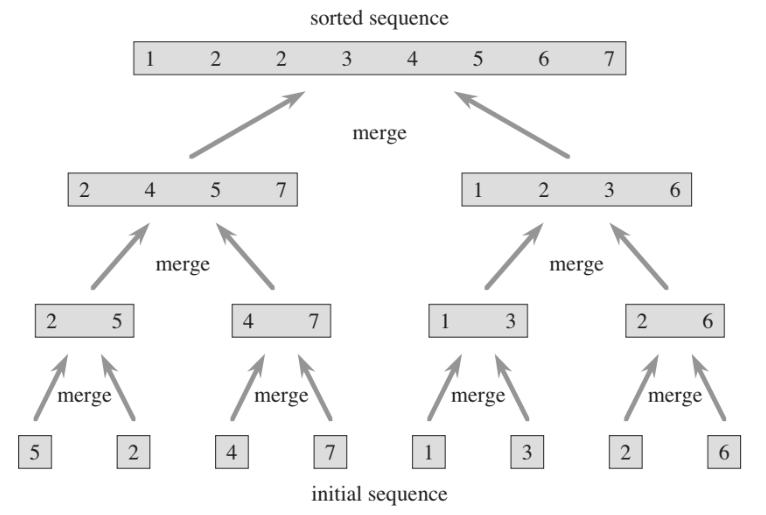
\includegraphics[scale=0.5]{merge}
\caption{
Merge sort being performed on an example array, note the figure starts with values already in single-element arrays.
}
\label{fig:merge_sort}
\end{figure}

Following figure 1, we get the $\log_2{n}$ by constantly splitting our arrays in half until we get to single-element arrays. The height of the tree is $\log_2{n} + 1$, times $n$ $c$'s, and adding each level up gives us $cn$, thus our total cost being $cn \log_2{n} + cn$, which is $\Theta{(n \log_2 n)}$. This is further illustrated by figure 2 at the end of the section.

\newpage
\section*{Recurrences}
Recurrences and the divide-and-conquer paradigm go hand in hand, because they provide a natural way to characterize the running time of divide-and-conquer algorithms. A \textbf{recurrence} is an equation or inequality that describes a function in terms of its value on smaller inputs. 
\\ \\
Recall merge sort's worst-case running time of $\Theta{(n\text{ log}_2(n))}$, it can be described by the following recurrence\\
$$
T(n)=
\begin{cases}
\Theta(1) & \text{if } n = 1,\\
2T(n/2) + \Theta{(n)} & \text{if } n > 1
\end{cases}
$$

Iterate to the solution, this is the iterative method to solve recurrences.\\
Given $n=2^k$, for some positive integer $k$.
\begin{equation*}
\begin{split}
  T(n) & = 2 \cdot T(n/2) + cn\\
  & = 2[2 \cdot T((n/2)/2) + c \cdot n/2] + cn = 2^2 \cdot T\bigg(\frac{n}{2^2}\bigg)+cn+cn\\
  & = 2^3 \cdot T\bigg(\frac{n}{2^3}\bigg)+cn+cn+cn\\
  & = 2^i \cdot T\bigg(\frac{n}{2^i}\bigg)+i \cdot cn\\
\end{split}
\end{equation*}
Recall $n=2^k$, let $k=\log_2{(n)}$, so let $i$ be $\log_2{(n)}$ or $k$. Thus,\\
\begin{equation*}
\begin{split}
  T(n) & = 2^k \cdot T\bigg(\frac{n}{2^k}\bigg) + k \cdot cn \text{\hspace{10mm}($i=k$), same thing}\\
  & = n \cdot T(1) + \log_2{(n)} \cdot cn\\
  & = n \cdot c + \log_2{(n)} \cdot cn \text{\hspace{10mm}(Recall $T(n=1) = c$)}\\
  & = (1 + \log_2{(n)}) \cdot cn\\
  T(n) & = cn + (1 + \log_2{(n)}) \text{ is the closed form solution.}
\end{split}
\end{equation*}

\begin{figure}[ht]
\centering
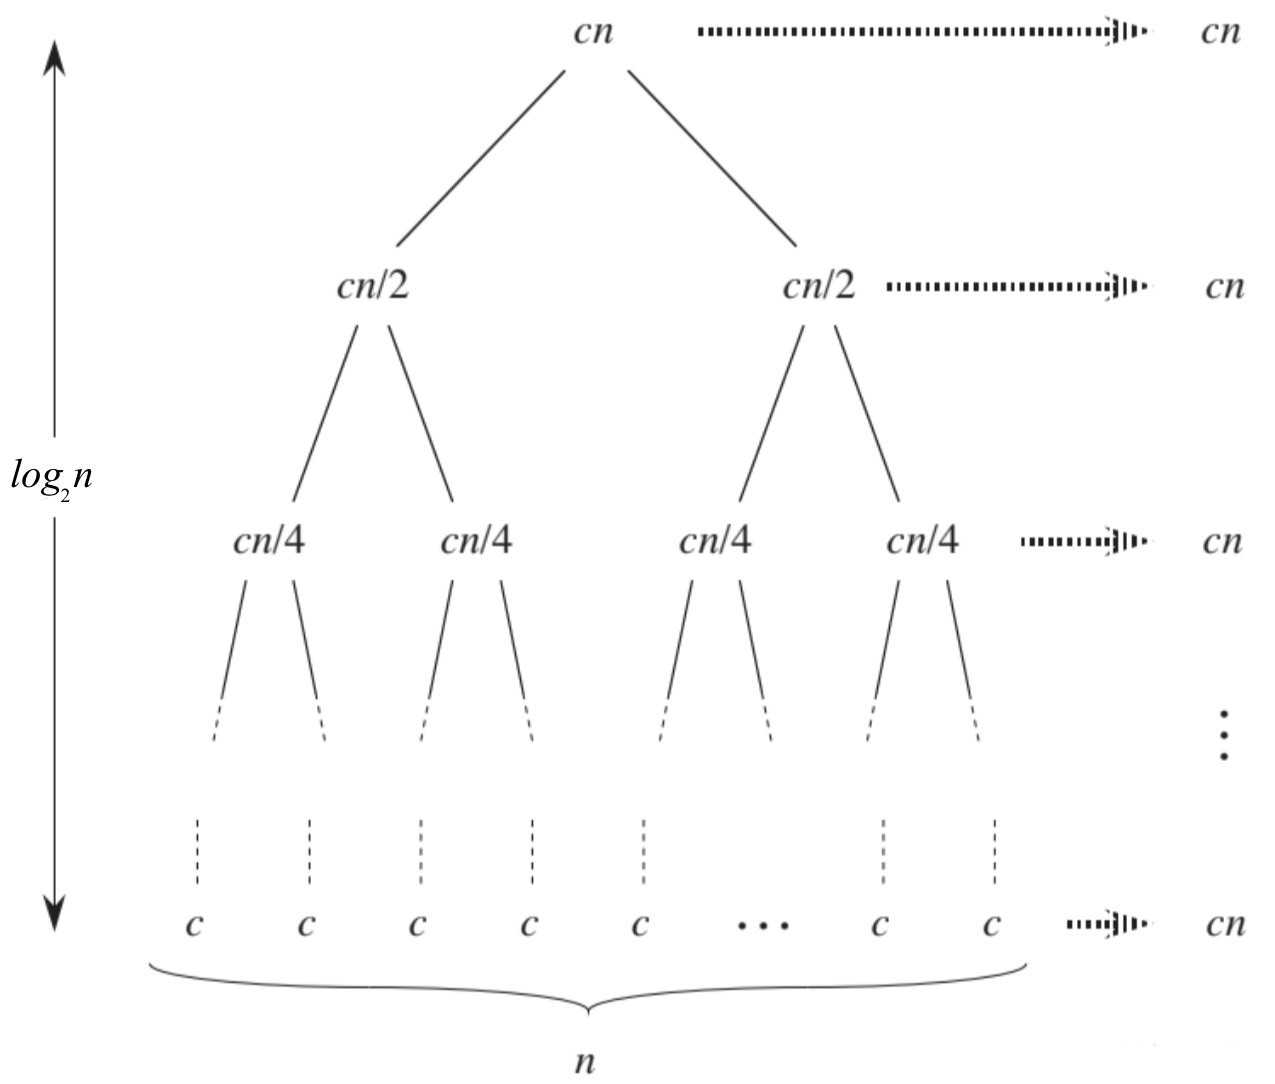
\includegraphics[scale=0.5]{merge_analysis}
\caption{
The recursion of merge sort visualized. The total height of the tree is $\log_2{n}$ and at each level $n$ costs which all equal $1*cn$, we also have $n$ number of $c$'s, adding $cn$ to the final running time of $cn\log_2{n} + cn$. This can be described by $\Theta{(n \log_2{(n)})}$ (the notation likes to exclude any constants).
}
\label{fig:merge_analysis}
\end{figure}
There are several ways to solve recurrences, the substitution and recursion tree methods involve guessing, so they are not the best ways to get solutions (which are the closed-form recurrences). The better methods are the iterative (worked out above) and the master theorem. 
\clearpage

\section*{The Master Theorem}
The master theorem applies to recurrences in the form\\
\begin{equation*}
    T(n) = aT\bigg(\frac{n}{b}\bigg) + f(n).
\end{equation*}

\textbf{Important things to remember:}
\begin{itemize}
    \item Every problem you recurse on should be the \textbf{same size}.
    \item There are $a$ subproblems, each of them of size $n/b$, with $f(n)$ recursive work.
\end{itemize}

\textbf{Constraints:}
\begin{itemize}
    \item $a \geq 1$ (at least one recursion).
    \item $b > 1$ (be able to make problem smaller).
    \item $f(n)$ must be asymptotically positive \\(positive for large enough $n$, $f(n) > 0$ for $n \geq n_0$.
\end{itemize}

\textbf{The three cases of the master theorem:}\\
Compare $f(n)$ with $n^{\log_b{a}}$.
\begin{itemize}
    \item \textbf{Case 1:} $f(n)$ is smaller.\\
        $f(n) = O{(n^{\log_b{a-\epsilon}})}$ for some epsilon $\epsilon > 0$.\\
        So, $f(n)$ will be polynomially smaller than $n^{\log_b{a}}$.\\
        $\Rightarrow T(n) = \Theta{\big(n^{\log_b{a}}\big)}$.
        
    \item \textbf{Case 2:} $f(n)$ is about the same (equal up to poly log factors).\\
        $f(n) = \Theta{\Big(n^{\log_b{a}} \cdot (\log_2{n})^k\Big)}$ for some $k \geq 0$.\\
        $\Rightarrow T(n) = \Theta{\Big(n^{\log_b{a}} \cdot (\log_2{n})^{k+1}\Big)}$.

    \item \textbf{Case 3:} $f(n)$ is polynomially bigger than $n^{\log_b{a}}$.\\
        $f(n) = \Omega{\Big(n^{\log_b{a+\epsilon}}\Big)}$ for some $\epsilon > 0.$\\
        We need another assumption about $f(n)$ because we are a bit more worried on how fast $f(n)$ grows.\\
        So,\\$a \cdot f\Big(\frac{n}{b}\Big) \leq c \cdot f(n)$ for some constant $c < 1$ and all sufficiently large $n$.\\
        $\Rightarrow T(n) = \Theta{(f(n))}$.
\end{itemize}

\end{document}
